\documentclass[a4paper]{article}

\input ../header
\usepackage{minted}
\usepackage[np]{numprint}
\usepackage{lscape}
\usepackage{afterpage}
\usepackage{hyperref}
\usepackage{gensymb}

\setlength{\multicolsep}{2pt}

% Commandes pour cacher/révéler du texte facilement à l'aide d'un booléen
\usepackage{xstring}
\usepackage{ifthen}

\newboolean{reveal}
\setboolean{reveal}{false}

\newlength{\stextwidth} % une nouvelle longueur

\newcommand\x{6}

\newcommand{\guess}[1]{\ifthenelse{\boolean{reveal}}{{\color{red}#1}}{\settowidth{\stextwidth}{#1}\makebox[\stextwidth]{\dotfill}}}

\newcommand{\guessmath}[1]{\ifthenelse{\boolean{reveal}}{\textcolor{red}{#1}}{\settowidth{\stextwidth}{$#1$}\makebox[1.9\stextwidth]{\dotfill}}}

\newcommand{\guessmathbin}[1]{\ifthenelse{\boolean{reveal}}{\mathbin{\color{red}#1}}{\settowidth{\stextwidth}{$#1$}\makebox[2\stextwidth]{\dotfill}}}

\begin{document}

\title{Chapitre 6 -- Géolocalisation}

\pagestyle{empty}

\date{}
\author{}

\maketitle{}

\thispagestyle{empty}
\noindent\textbf{Activité 4}\hfill{}\textbf{Manifestation}
\smallskip
\hrule
\medskip

 La géolocalisation associe un système global de positionnement (type GPS), un système géodésique (type WGS84) et un système d'information géographique qui permet de visualiser sa position sur une carte.

 \medskip

 \begin{multicols}{2}
   \begin{center}
     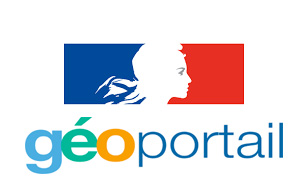
\includegraphics[width=5cm]{logo-geoportail.jpg}
   \end{center}\columnbreak 

   \vspace*{-1mm}

 La plateforme Geoportail (\url{https://www.geoportail.gouv.fr/}) mise en oeuvre par l'Institut National de l'information Géographique et forestière (IGN), a pour vocation de faciliter l'accès à l'information géographique de référence.
 \end{multicols}

 \begin{multicols}{2}
   \vspace*{-1mm}
   Le 9 janvier 2020, une manifestation contre la réforme des retraite a eu lieu en France. À:w
   Paris, \np{56 000} personnes ont manifesté, selon le ministère de l’Intérieur, \np{370 000} selon la CGT (syndicat).

   \medskip 

   Le cortège avait pour point de départ \textit{Place de la République }et pour arrivée \textit{Place de la Concorde} à Paris. 

   \medskip 

   La photo ci-contre donne une vue aérienne du rassemblement. 
   \vspace*{3cm}
   \begin{center}
     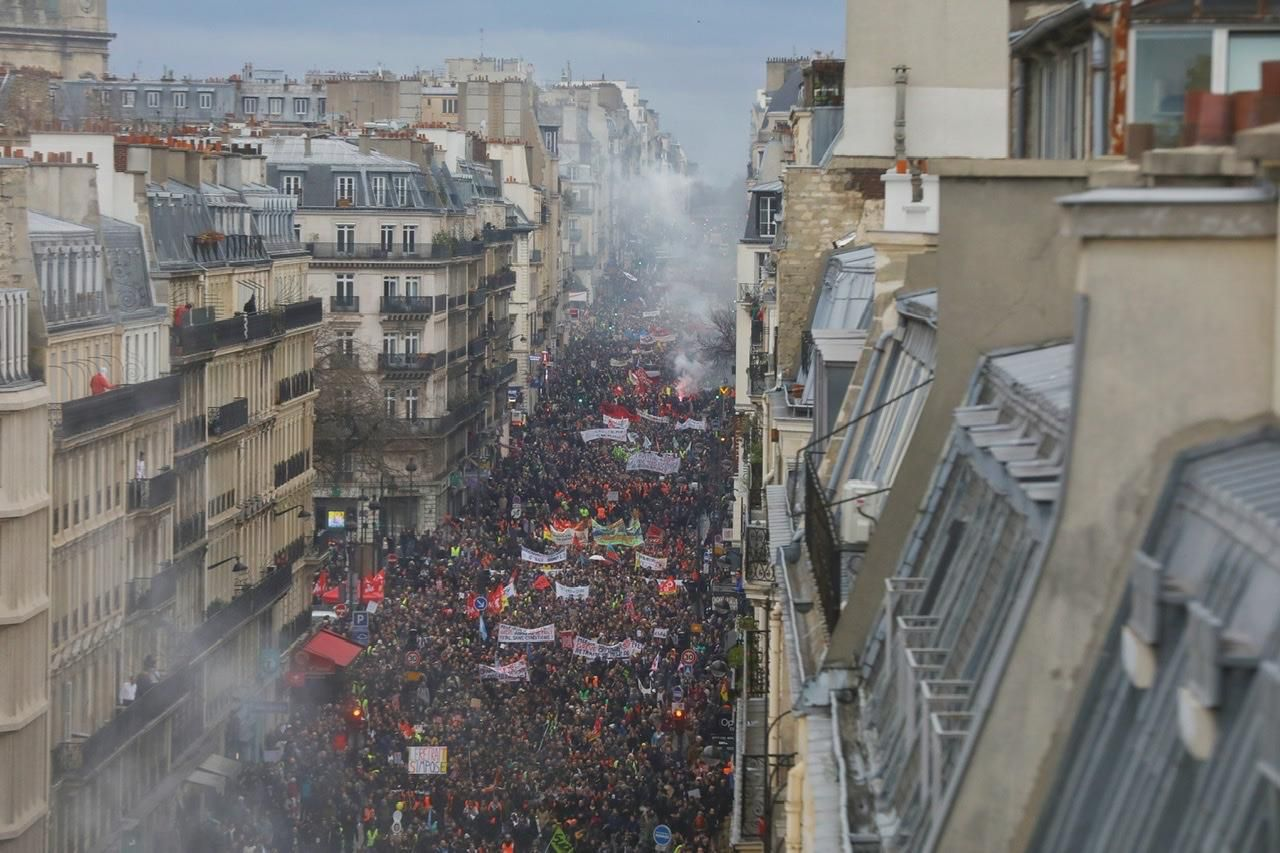
\includegraphics[width = 7cm]{cortege_manifestation.jpg}
   \end{center}
 \end{multicols}

      \begin{enumerate}
	\item Ouvrir un navigateur web et se rendre sur la plateforme \href{https://www.geoportail.gouv.fr/}{https://www.geoportail.gouv.fr/}. 
	\item Rechercher les lieux suivants (à Paris) : \textit{Place de la République} et \textit{Place de la Concorde}. 

	  \textit{On pourra utiliser la recherche avancé par adresse.}

	  À l'aide des outils principaux de la barre d'outils, on placera un repère sur chacun de ces lieux. 
	\item À l'aide des outils principaux de la barre d'outils, calculer l'itinéraire de la \textit{Place de la République} à la \textit{Place de la Concorde} à pied via le chemin le plus rapide.

	  \begin{center}
	    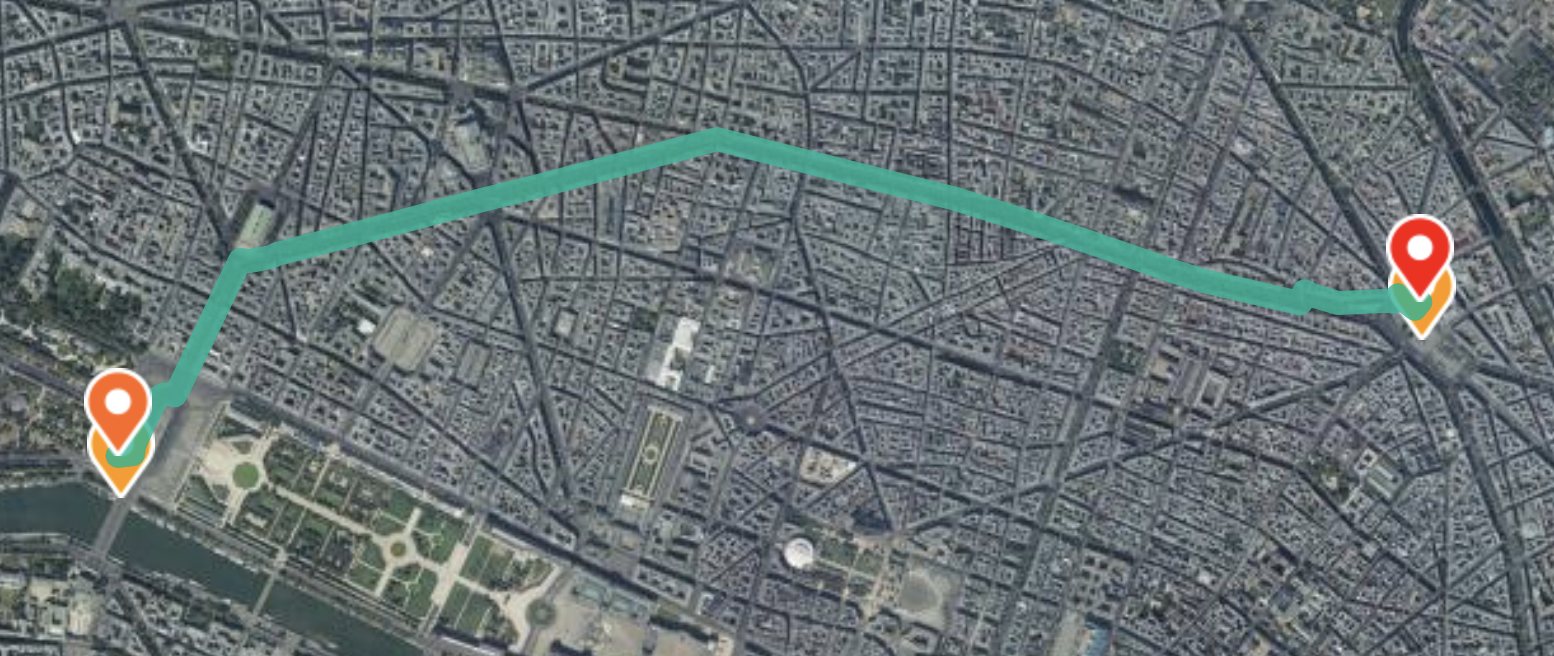
\includegraphics[width = 12cm]{itineraire.png}
	  \end{center}


	  \medskip 

	  \dotfill\rep{3}

	  %{\color{blue} On obtient \np{3,68} km et 54 min.
	  %}


	\item 

	  \begin{enumerate}
	    \pagebreak
	    \item À l'aide des outils de mesure, établir un \textit{profil altimétrique} de l'itinéraire du parcours. 

	      {\color{blue}
		\begin{center}
		  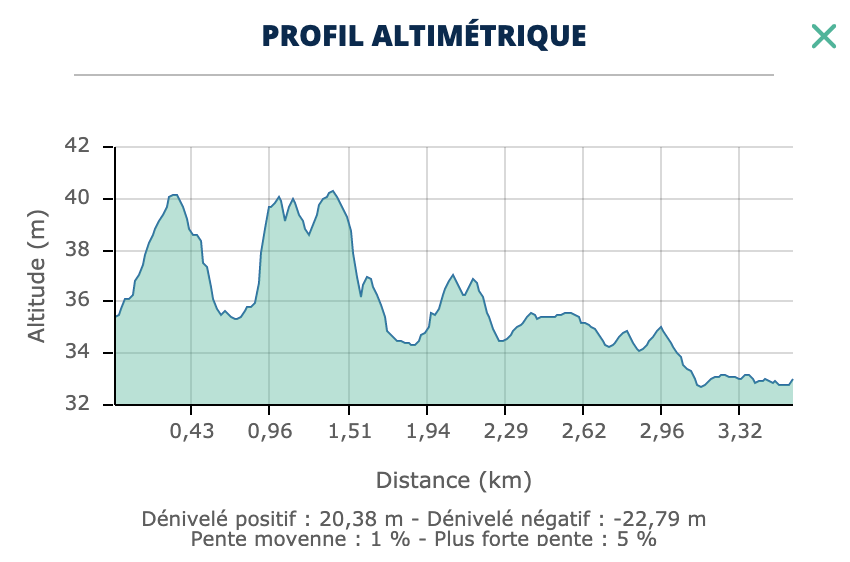
\includegraphics[width = 10cm]{altimetrie.png}
		\end{center}
	      }
	    \item Selon vous, faut-il être un sportif confirmé pour effectuer ce parcours ? 

	      %  {\color{blue} Non pas du tout, la pente est très légère tout au long du parcours. }

	      \medskip 

	      \dotfill 


	  \end{enumerate}

	\item Positionnez-vous au niveau du \textit{14 boulevard des Capucines}, dans votre itinéraire, avec une échelle de $1:750$.
	  À l'aide des outils de mesure, calculer la surface du boulevard sur 100 mètres.\rep{2}

	  {\color{blue} 
	    \begin{center}
	      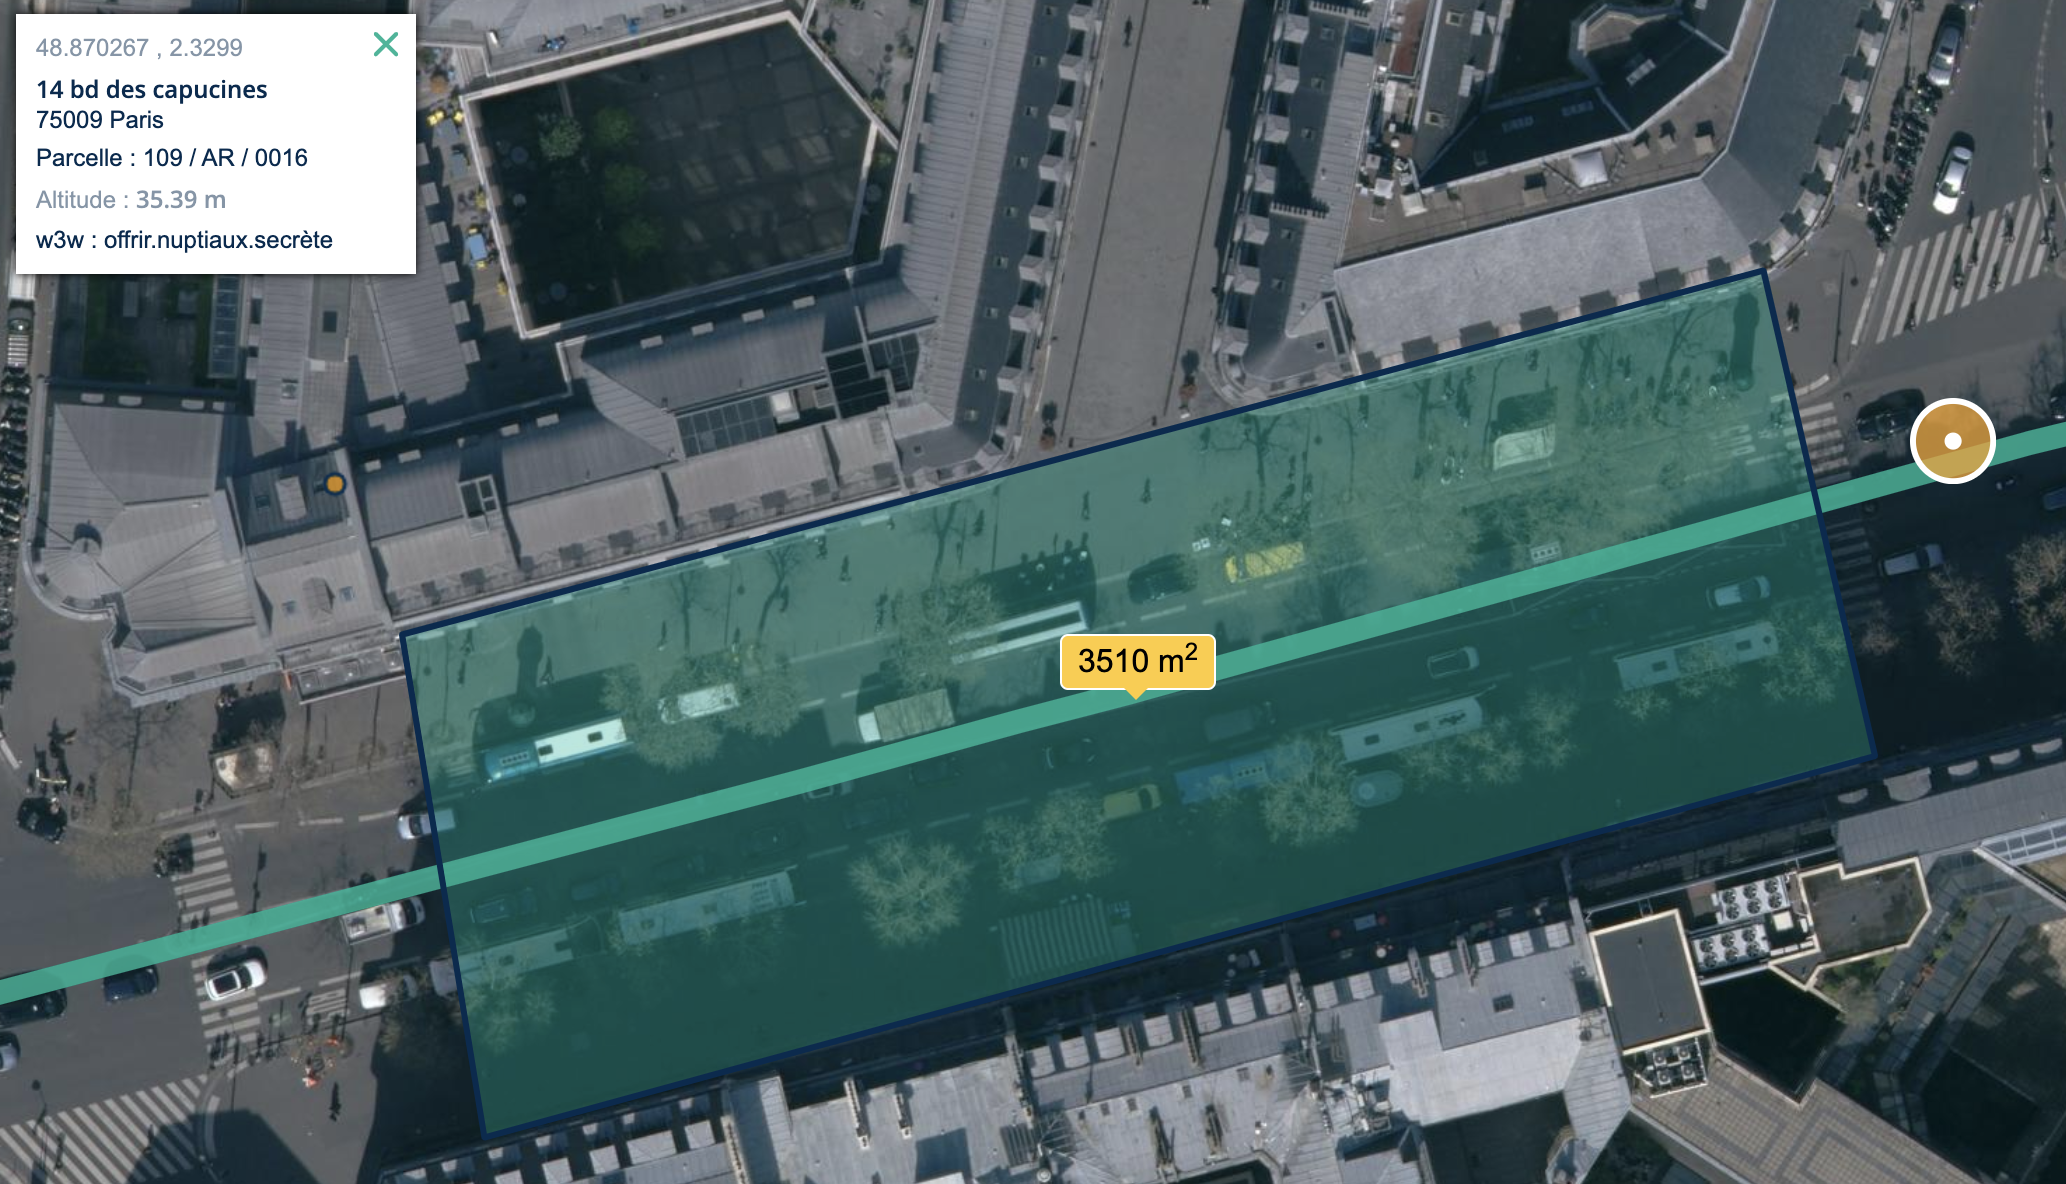
\includegraphics[width = 10cm]{surface.png}
	    \end{center}
	  }


	\item En supposant qu'il y a environ un manifestant au mètre carré et que la largeur du boulevard est constant tout au long de l'itinéraire.
	  \begin{enumerate}
	    \item Selon l'estimation faite par le ministère de l'intérieur, sur combien de mètres s'étend le cortège ? \rep{4}

	      %		{\color{blue}
	      %		D'après la question précédente, sur 100m, il y a environ \np{3510} manifestants. 
	      %		
	      %		Donc \np{56 000} manifestants occupent une surface de \np{56 000} $m^2$, ce qui donne une longueur de cortège de : 
	      %		
	      %		\[\dfrac{\np{56000}}{3510}\times 100 \approx \np{1595} \, \mbox{m  soit } 1,595 \mbox{ km}\]
	      %		}

	      
	    \item Selon l'estimation faite par le syndicat, sur combien de mètres s'étend le cortège ? \rep{4}

	      %		{\color{blue}
	      %		D'après la question précédente, sur 100m, il y a environ \np{3510} manifestants. 
	      %		
	      %		Donc \np{370 000} manifestants occupent une surface de \np{370 000} $m^2$, ce qui donne une longueur de cortège de : 
	      %		
	      %		\[\dfrac{\np{370 000}}{3510}\times 100 \approx \np{10541} \, \mbox{m  soit } 10,541 \mbox{ km}\]
	      %		}

	      

	    \item Expliquer pourquoi le décompte du syndicat ne semble pas cohérent. \rep{4}

	      %		{\color{blue} L'itinéraire de la manifestation fait \np{3,68} km alors que la longueur estimé du cortège fait $10,541$ km. 
	      %		
	      %		}
	      
	  \end{enumerate}

	\item En supposant que la longueur du cortège est égale à la longueur de l'itinéraire du parcours. 

	  Quelle serait la densité de manifestant au mètre carré selon le syndicat ? \rep{4}


	  %        {\color{blue} La surface totale de l'itinéraire est donnée par : 
	  %        
	  %        \[\np{3680} \times \dfrac{3510}{100} = \np{129168} \mbox{ m}^2\]
	  %        
	  %        Donc, le nombre de manifestant au mètre carré est donné par : 
	  %        
	  %        \[\dfrac{\np{370000}}{\np{129168}} \approx 3 \mbox{ manifestants/m}^2\]
	  %        
	  %        }
      \end{enumerate} 

\end{document}
